\mode*

\section{Kurven: Pfade und Wege}

%%%%%%%%%%%%%%%%%%%%%%%%%%%%%%%%%%%%%%%%%%%%%%%%%%%%%%%%%%%%
\begin{frame}
    \begin{Denkpause}
        Auf einer Wanderung bewegen Sie sich durch eine Landschaft. Was für ein mathematisches Objekt ist geeignet, diese Bewegung zu beschreiben.
    \end{Denkpause}
\end{frame}

\begin{frame}{Definition: Weg}
    Ein Weg ist eine Abbildung von einem Zeitintervall $I$ in einen Vektorraum, zum Beispiel $\R^n$.
\end{frame}
%%%%%%%%%%%%%%%%%%%%%%%%%%%%%%%%%%%%%%%%%%%%%%%%%%%%%%%%%%%%
\begin{frame}{Analytische Eigenschaften von Pfaden}
    \begin{itemize}
        \item Stetigkeit, Differenzierbarkeit und Integrale von Pfaden sind komponentenweise definiert.
        \item Ableitungen
        \begin{gather*}
            \vf'(t) = \tfrac{d}{dt}
            \begin{pmatrix}
                \tfrac{d}{dt} f_1(t)\\
                \vdots\\
                \tfrac{d}{dt} f_n(t)
            \end{pmatrix}
            = \begin{pmatrix}
                f_1'(t)\\\vdots\\f_n'(t)
            \end{pmatrix}
        \end{gather*}
        \item Integrale
        \begin{gather*}
            \int \vf(t)\,dt = \vF(t),
        \qquad F_i(t) = \int f_i(t)\,dt,\quad i=1,\dots,n
        \end{gather*}
    \end{itemize}
\end{frame}

%%%%%%%%%%%%%%%%%%%%%%%%%%%%%%%%%%%%%%%%%%%%%%%%%%%%%%%%%%%%
\begin{frame}{Beispiele in zwei Dimensionen}
    \begin{columns}
        \begin{column}[t]{.5\textwidth}
        \begin{block}{Geradlinige Bewegung}
            \begin{align*}
                x(t) &= f_1(t) = x_0 + t u\\
                y(t) &= f_2(t) = y_0+tv
            \end{align*}
            oder in Vektorschreibweise
            \begin{gather*}
                \vx(t) = \vx_0+t\vv
            \end{gather*}
            Ableitung
            \begin{gather*}
                \vx'(t) = \vv
            \end{gather*}
        \end{block}         
        \end{column}
        \pause
        \begin{column}[t]{.5\textwidth}
        \begin{block}{Kreisbewegung}
            \begin{align*}
                x(t) &= r \cos t\\
                y(t) &= r \sin t
            \end{align*}
            mit der Ableitung
            \begin{align*}
                x(t) &= -r \sin t\\
                y(t) &= r \cos t
            \end{align*}
        \end{block}         
        \end{column}
    \end{columns}
\end{frame}

%%%%%%%%%%%%%%%%%%%%%%%%%%%%%%%%%%%%%%%%%%%%%%%%%%%%%%%%%%%%
\begin{frame}{Definition Weg}
\mrerror{Warum wird "Weg" nochmal definiert, wenn dies bereits in 2.0.1 geschieht?}    
\end{frame}

\begin{envgknote}{hinzufügen}
   \begin{itemize}
       \item Wege: parametrische und nullstellen-Darstellung
       \item Begriffsklärung
       \item Beispiele Gerade und Kreis
       \item zu einem Weg kann es mehrere Pfade geben, die ihn parametrisieren
       \item Beispiel chemische Reaktion oder Biosystem
       \item Wann ist ein Weg als $y=f(x)$ darstellbar?
       \item Implizite Differentiation
   \end{itemize} 
\end{envgknote}

\mrnote{Folgende passenden Folien sind provisorisch aus der alten Vorlesung entnommen:}

%%%%%%%%%%%%%%%%%%%%%%%%%%%%%%%%%%%%%%%%%%%%%%%%%%%%%
\begin{frame}
    \frametitle{Darstellung eines Weges als Funktion}

    Unter welchen Bedingungen lässt sich ein Weg auch als \grqq klassischer \grqq Graph einer Funktion $y=f(x)$ betrachten?

    \begin{itemize}
        \item Bewegung eines Punktes auf einen festen Kreis
    \begin{columns}
        \begin{column}{0.5\textwidth}
    $$
    \left\{\begin{array}{l}
        x(t) = a\cos(\omega t)\\ y(t) = a\sin(\omega t)
    \end{array}\right.
    $$
\end{column}
\begin{column}{0.5\textwidth}
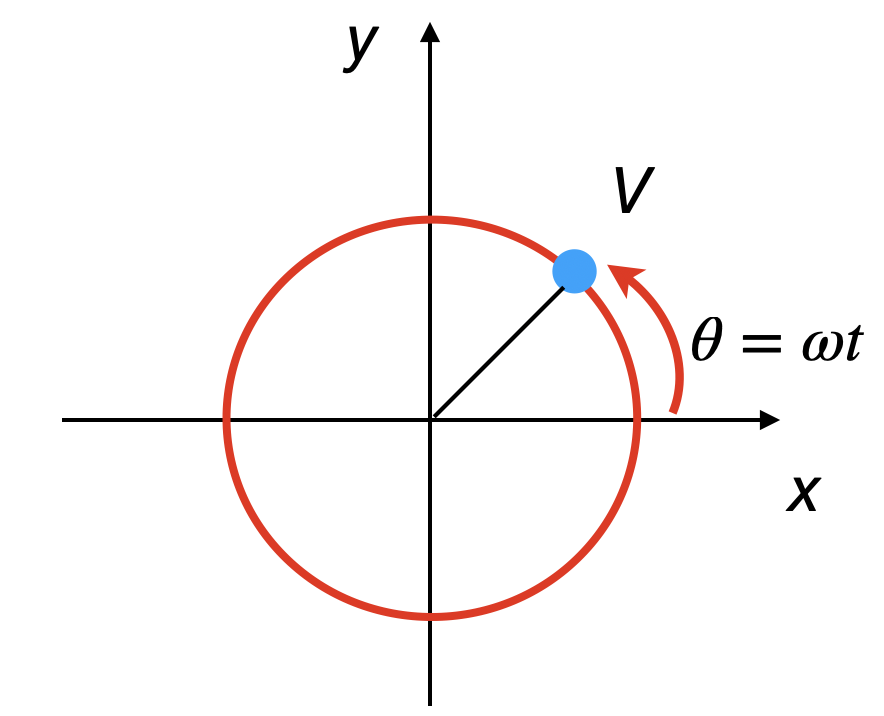
\includegraphics[width=0.5\textwidth]{fig/pk03.png}
\end{column}
\end{columns}
    \item $\sin(\omega t) = \sqrt{1-\cos^2(\omega t)}$ (nur für die obere Kreishälfte!)
    \item Daher:
    \begin{multline}
    y(t) = a\sin(\omega t) \Longrightarrow y(t) = a \sqrt{1-\cos^2(\omega t)} \\ 
    \Longrightarrow y(t) = \sqrt{a^2-a^2\cos^2(\omega t)} \Longrightarrow y(t) = \sqrt{a^2-x(t)^2} 
    \end{multline}
    \item Also: $y = f(x) = \sqrt{a^2-x^2}$ (obere Kreishälfte)
\end{itemize}


\end{frame}

\mode<all>
